\begin{frame}[plain]
\frametitle{Perspectiva general}
%------------------------------
\begin{columns}

    \pgfsetfillopacity{0.2}

    \begin{column}{0.50\textwidth}
    \vspace{-5pt}
    \begin{block}{\textcolor{blue}{Oferta}}
        \begin{column}{0.1\textwidth}
        \vspace{-10pt} % estos espacios negativos son claves para alinear
            \tiny
            \begin{align*}
            c_{1,t}+\Phi_t \le y\\
            c_{2,t+1}\le\Phi_{t+1}^R\\
            N_{t-1}\textcolor{red}{x_t} \cdot \Phi_{t-1}^{\textbf{DLT}}=N_t(*)
            \end{align*}
        \end{column}
        \begin{column}{0.35\textwidth}  
            \begin{figure}[H]
            \begin{center}
             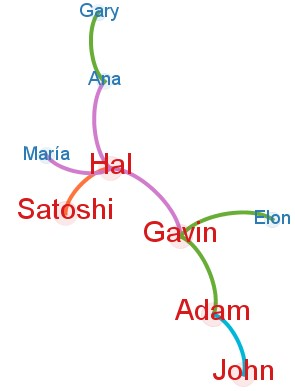
\includegraphics[width=1\textwidth]{images/C2/c2_simul_red5.jpg}
             \end{center}
            \end{figure}
            \end{column}
    \end{block}
    
    \begin{block}{\textcolor{dgreen}{Demanda}}
        \vspace{-10pt}
            \tiny
              \begin{align*}
              v_{t}^{\$}{M_{t}^{\$}}&={N_{t}^{\$}\left(*\right)}+(1-\lambda_t){N_{t}^{\$}\left(*\right)}\\
              v_{t}^{\bitcoinA}{M_{t}^{\bitcoinA}}&={N_{t}^{\bitcoinA}\left(*\right)+\lambda_tN_{t}^{\$}\left(*\right)}\\
              \lambda_t&=\textcolor{blue!70}{S}(\textcolor{red}{\mu_t})
            \end{align*}
    \vspace{-20pt}
            \begin{figure}[t!]
            \begin{center}
            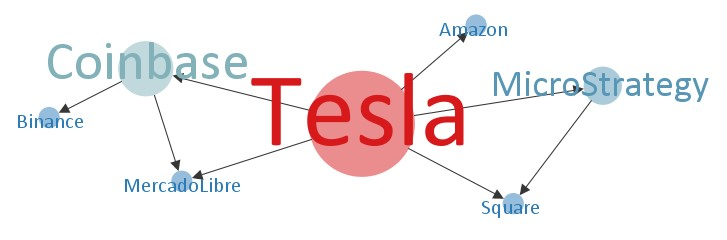
\includegraphics[width=0.6\textwidth]{images/C3/c3_simul_influ3.jpg}
             \end{center}
            \end{figure}
            
    \end{block}
    \end{column}
    
    \begin{column}{0.55\textwidth}
    
    \pgfsetfillopacity{1}
    
    \begin{block}{\textcolor{orange}{Implicancias}}
    \tiny

    \begin{align*}
    v^{\$a}_1 M^{\$a}_1&=P_1^{{\$a}} + \lambda_1 (1-\alpha_1) R_1^{{\$a}} + (1-\lambda_1){\rho_1}  R_1^{{\$a}}\\
    v_1^{\$} M_1^{\$}&=(1-\lambda_1) \textcolor{green!70}{\delta_1} R_1^{\$a}\\
    v_1^{\bitcoinA} M_1^{\bitcoinA}&={\lambda_1}  \alpha_1 R_1^{\$a} + (1-\lambda_1){\beta_1} R_1^{\$a}\\
    e_t^{{\$a};{\$}}&=\frac{v_1^{\$a}}{v_1^{\$}}
    \end{align*}
    
    \vspace{-5pt}
    
    \begin{figure}[H]
    \begin{center}
     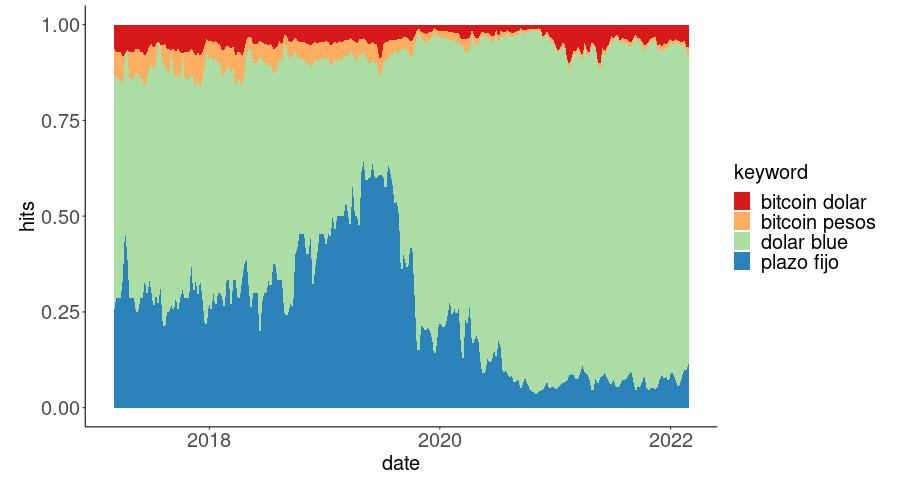
\includegraphics[width=1\textwidth]{images/C4/Rplot001.png}
     \end{center}
    \end{figure}
    
    \end{block}

    \end{column}
\end{columns}

\note{
\begin{itemize}
    \item Finalizada la primera y segunda parte de la investigación, volvemos a la filmina que presenta el panorama general. 
    \item Ahora vamos a comenzar con la última parte de la investigación asociada a las implicancias de una mayor adopción de bitcoin en Argentina. 
\end{itemize}
}

\end{frame}
%----------

\subsection{Objetivos}
%---------------------
\begin{frame}{}

    \textcolor{blue}{\textbf{Objetivo}}.\\
    \vspace{5mm}
    \begin{itemize}
        \setlength\itemsep{1em}
        \item[] Analizar los riesgos para la estabilidad financiera asociados a bitcoin en una economía emergente. 
        \item[] Construir un \textcolor{blue}{modelo} que explique las consecuencias de un incremento en la \textcolor{blue}{volatilidad de demanda de bitcoin} en el nivel del \textcolor{blue}{tipo de cambio} entre pesos y dólares en Argentina.
        \item[] \textcolor{blue}{Evaluar empíricamente} el modelo propuesto a partir de datos estimados para Argentina.
    \end{itemize}
 
    \vspace{5mm}
    \textcolor{dgreen}{\textbf{Conjetura}}. 
    \vspace{5mm}
    \begin{itemize}
    \item[] Incrementos en la  \textcolor{dgreen}{volatilidad de la demanda de bitcoin} pueden generar incrementos en la  \textcolor{dgreen}{volatilidad en el tipo de cambio} entre pesos y dólares.
    \end{itemize}

\note{
\begin{itemize}
    \item Para esta tercera y última parte de la investigación, se plantean los siguientes tres objetivos específicos
    \item (Leer cada objetivo)
    \item A su vez, se plantea una última conjetura:
    \item (Leer la conjetura)
\end{itemize}
}
    
\end{frame}
%----------

\subsection{Definiciones}
%------------------------
\begin{frame}

\vspace{5mm}
\begin{displayquote}
\textcolor{blue}{Sustitución de monedas} se define como el uso en un país determinado de múltiples monedas como \textcolor{blue}{medio de cambio}. 
\end{displayquote}

\vspace{5mm}
\begin{displayquote}
El término \textcolor{dgreen}{dolarización} también se utiliza con frecuencia para indicar que una moneda extranjera sirve como unidad de cuenta o como \textcolor{dgreen}{depósito de valor}, y no necesariamente como medio de cambio.
\end{displayquote}
\vspace{5mm}
\raggedleft \cite{Calvo1992}\\ \citetitle{Calvo1992}

\note{
\begin{itemize}
    \item Para esta tercera parte de la investigación se propone retomar algunos conceptos asociados a la sustitución de activos monetarios.
    \item En este sentido, \textbf{Calvo y Vegh} proponen dos definiciones complementarias (leer citas)
    \item Esta distinción entre sustitución de activos como medios de pago o como reserva de valor será relevante para la presente parte de la investigación.  
\end{itemize}
}
    
\end{frame}
%----------

\subsection{Evaluación conceptual y empírica}
%-----------------------------------------------

% overwiew
\begin{frame}[t]
\frametitle{Evaluación conceptual y empírica}
    
    \begin{block}{Modelo}
        \vspace{-10pt}
        \begin{column}{0.4\textwidth}
            \tiny
            \begin{align*}
            v^{\$a}_1 M^{\$a}_1&=P_1^{{\$a}} + \lambda_1 (1-\alpha_1) R_1^{{\$a}} + (1-\lambda_1){\rho_1}  R_1^{{\$a}}\\
            v_1^{\$} M_1^{\$}&=(1-\lambda_1){\delta_1} R_1^{\$a}\\
            v_1^{\bitcoinA} M_1^{\bitcoinA}&={\lambda_1}  \alpha_1 R_1^{\$a} + (1-\lambda_1){\beta_1} R_1^{\$a}\\
            e_t^{{\$a};{\$}}&=\frac{v_1^{\$a}}{v_1^{\$}}
            \end{align*}
        \end{column}
        \begin{column}{0.4\textwidth}
        \end{column}
    \end{block}
    
\begin{block}{Evaluación empírica}
    
    \begin{minipage}[t][.4\textheight][t]{\textwidth}
        
        \begin{column}{0.5\textwidth}
    \tiny
    \begin{figure}[H]
        \begin{center}
             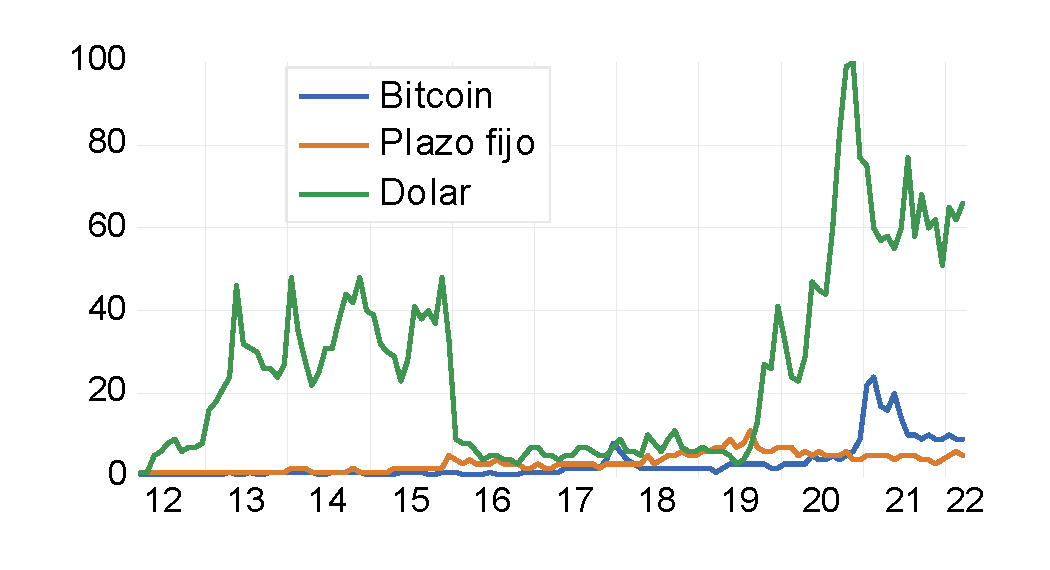
\includegraphics[width=1\textwidth]{images/C4/times_series_gtrend_tot.pdf} % búsqueda general timeseries
         \end{center}
    \end{figure}
    \end{column}
    \begin{column}{0.5\textwidth}  
    \tiny
    \begin{figure}[H]
        \begin{center}
         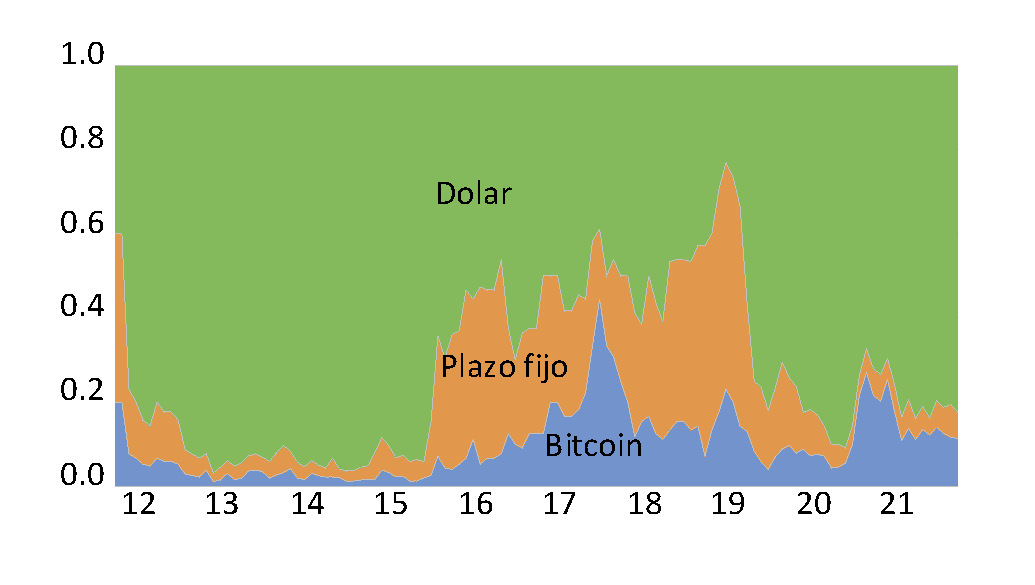
\includegraphics[width=1\textwidth]{images/C4/spike_gtrend_tot.pdf} % búsqueda general spike
        \end{center}
        
        \end{figure}
\end{column}

    \end{minipage}
\end{block}

\note{
\begin{itemize}
    \item Para la evaluación conceptual se continúa con el modelo de las secciones anteriores. Ahora se incorpora un nuevo activo: un activo fiduciario externo. 
    \item Para evaluar empíricamente se construye una base de datos con las búsuqedas de los argentinos de términos asociados a los activos monetarios propuestos en el modelo. 
\end{itemize}
}
    
\end{frame}

% slides primera parte (ev conceptual)
\begin{frame}[t]
\frametitle{Evaluación conceptual y empírica}
    
    \begin{block}{Modelo}
        \vspace{-10pt}
        \begin{column}{0.3\textwidth}
            \tiny
            \begin{align*}
            % mercado de pesos
            \onslide<1-3,4,5,6,7>{v^{\$a}_1 M^{\$a}_1}&=
            \onslide<2,6>{P_1^{{\$a}}} 
            \onslide<4,6,7>{+ \lambda_1 (1-\alpha_1)} 
            \onslide<3,4,6,7>{R_1^{{\$a}}} 
            \onslide<5-6>{+ (1-\lambda_1) \rho_1}
            \onslide<3,5-6>{R_1^{{\$a}}}
            \\ % mercado de dólares
            \onslide<1,3,5,6>{v_1^{\$} M_1^{\$}}&=
            \onslide<5,6,8>{(1-\lambda_1) \delta_1}
            \onslide<3,5,6,8>{R_1^{\$a}}
            \\ % mercado de bitcoin
            \onslide<1,3,4,5,6>{v_1^{\bitcoinA} M_1^{\bitcoinA}}&=
            \onslide<4,6,7>{\lambda_1 \alpha_1}  
            \onslide<3,4,6,7>{R_1^{\$a}} 
            \onslide<5,6,8>{+ (1-\lambda_1) \beta_1}
             \onslide<3,
             5-6>{R_1^{\$a}}
            \\ % tipo de cambio
            \onslide<7,8>{e_t^{{\$a};{\$}}&=\frac{v_1^{\$a}}{v_1^{\$}}}
            \end{align*}
        \end{column}
        \begin{column}{0.46\textwidth}
        \only<1|handout:0>{
                    \tiny
                    \justify
                    Oferta:
                    \begin{itemize}
                        \item $v_t$: valor de una unidad del activo monetario en término de bienes;
                        \item $M_t$: oferta de activos monetarios.
                    \end{itemize}
                    }
        \only<2-6|handout:0>{
        \begin{table}
        \renewcommand{\arraystretch}{1.5} 
        \tiny
        \only<2>{$P_1^{\$a}$: demanda para pagos}
        \only<3>{$R_1^{\$a}$: demanda como reserva}
        \only<4>{$R_1^{\$a}$: demanda como reserva rest.}
        \only<5>{$R_1^{\$a}$: demanda como reserva s/rest.}
        \centering
        \begin{threeparttable}
        \begin{tabular}{l|c|c|c|c|c|c|} 
        \cline{2-7}
                  & \multicolumn{6}{c|}{$N_t^{\$a}(y^{\$a}-c_{1,t}^{\$a})$}                                      \\ 
        \cline{2-7}
        \multirow{3}{*}{} & \multirow{3}{*}{\onslide<2,6>{$I$}} & \multicolumn{5}{c|}{\onslide<3-6>{$(1-I)$}}                                       \\ 
        \cline{3-7}
                  &                       & \multicolumn{2}{c|}{\onslide<4,6>{$\lambda$}} & \multicolumn{3}{c|}{\onslide<5-6>{$(1-\lambda)$}}  \\ 
        \cline{3-7}
                  &                       & \onslide<4,6>{$\alpha$} & \onslide<4,6>{$(1-\alpha)$}      & \onslide<5,6>{$\rho$} & \onslide<5,6>{$\delta$} & \onslide<5,6>{$\beta$}   \\
        \cline{2-7}
        \end{tabular}
        \end{threeparttable}
        \end{table}
                        }
  
        \only<7|handout:0>{
                    \tiny
                    \justify
                    Tipo de cambio:
                    \begin{itemize}
                        \item Si $\uparrow \alpha_t \downarrow v^{\$a}_t \downarrow e_t^{{\$a};{\$}}$ 
                        \end{itemize}
                    }
        
        \only<8|handout:0>{
                    \tiny
                    \justify
                    Tipo de cambio:
                    \begin{itemize}
                        \item Si $\uparrow \beta_t \downarrow \delta_t \downarrow v^{\$}_t \uparrow e_t^{{\$a};{\$}}$ 
                        \end{itemize}
                    }
        
        \end{column}
    \end{block}
    
\begin{block}{Evaluación empírica}
    
    \begin{minipage}[t][.4\textheight][t]{\textwidth}
       \end{minipage}
\end{block}

\note{
\footnotesize
\begin{itemize}
    \item Se define una economía emergente con tres activos monetarios: ARS, USD y BTC. 
    \item Se define una oferta local para cada uno de los tres activos
    \item La demanda del país emergente se va a particionar en diferentes demandas a partir de las restricciones del gobierno y de las preferencias de los individuos. 
    \item En primer lugar de define una demanda para realizar pagos (posiblemente asociada a la posibilidad de pagar impuestos con moneda local). Esta demanda para pagos se asocia al activo local pesos (solo aparece en la primera línea de las ecuaciones)
    \item Luego se define una demanda como reserva de valor. 
    \item Que depende de las restricciones a la tenencia de dólares (solo se puede elegir entre pesos y bitcoin)
    \item Mientras que los ciudadanos no alcanzados por las restricciones pueden elegir entre cualquier de los tres activos como reserva
    \end{itemize}
}
    
\end{frame}
%----------

% slides primera parte (ev empírica volatilidad)
\begin{frame}[t]
\frametitle{Evaluación conceptual y empírica}
    
    \begin{block}{Modelo}
        \vspace{-10pt}
        \begin{column}{0.4\textwidth}
            \tiny
            \begin{align*}
            v^{\$a}_1 M^{\$a}_1&=P_1^{{\$a}} + \lambda_1 (1-\alpha_1) R_1^{{\$a}} + (1-\lambda_1) {\rho_1}  R_1^{{\$a}}\\
            v_1^{\$} M_1^{\$}&=(1-\lambda_1){\delta_1} R_1^{\$a}\\
            v_1^{\bitcoinA} M_1^{\bitcoinA}&={\lambda_1}  \alpha_1 R_1^{\$a} + (1-\lambda_1){\beta_1} R_1^{\$a}\\
            e_t^{{\$a};{\$}}&=\frac{v_1^{\$a}}{v_1^{\$}}
            \end{align*}
        \end{column}
        \begin{column}{0.4\textwidth}
        \end{column}
    \end{block}
    
\begin{block}{Evaluación empírica}
    
    \begin{minipage}[t][.4\textheight][t]{\textwidth}
                    
        
        \begin{column}{0.5\textwidth}
    \tiny
    \begin{figure}[H]
        \begin{center}
             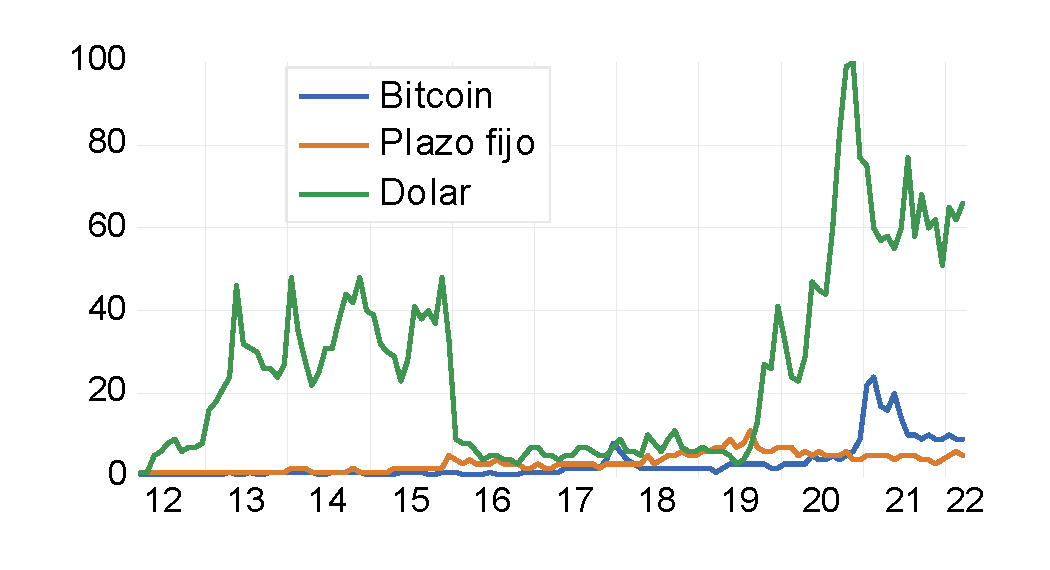
\includegraphics[width=1\textwidth]{images/C4/times_series_gtrend_tot.pdf} % búsqueda general timeseries
         \end{center}
    \end{figure}
    \end{column}
    \begin{column}{0.5\textwidth}  
    \tiny
    \begin{figure}[H]
        \begin{center}
         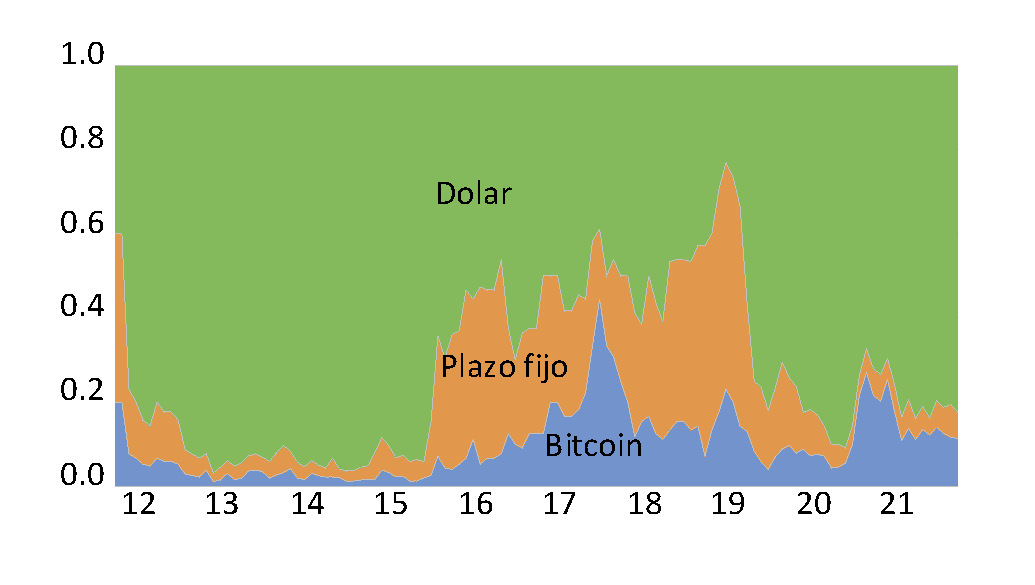
\includegraphics[width=1\textwidth]{images/C4/spike_gtrend_tot.pdf} % búsqueda general spike
        \end{center}
        
        \end{figure}
\end{column}

    \end{minipage}
\end{block}

\note{
\begin{itemize}
    \item La evaluación empírica tiene por objetivo principal estimar si la volatilidad en la demanda de bitcoin se traslada a volatilidad en el tipo de cambio entre ARSUSD. 
    \item Debido a que no se cuenta con datos oficiales de proveedores de bitcoin en Argentina, se construye una base de datos con las búsquedas de los términos bitcoin, dolar y plazo fijo en google. 
    \item Se observa un incremento en las búsquedas de la palabra bitcoin en los últimos años. 
\end{itemize}
}
    
\end{frame}

\begin{frame}
\frametitle{Se compara la volatilidad en las búsquedas}

\begin{figure}[H]
    \begin{center}
         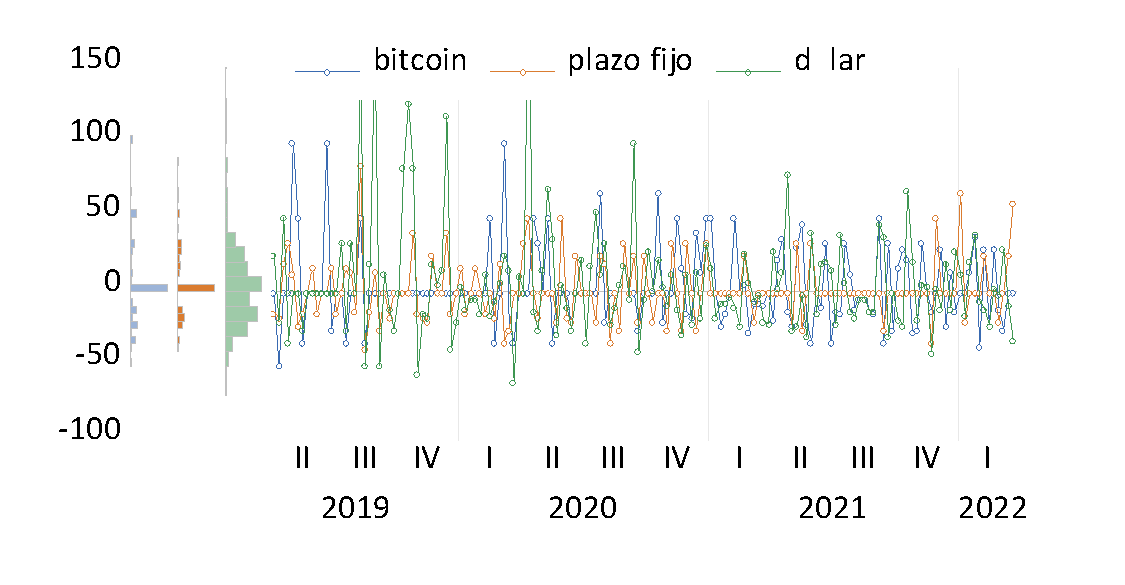
\includegraphics[width=1\textwidth]{images/C4/vol/vol_gtrends_20192022.pdf}
     \end{center}
\end{figure}

\note{
\begin{itemize}
    \item Al estimar la volatilidad en las búsquedas de los términos, no se encuentra mayor volatilidad en las búsquedas de bitcoin que en las búsquedas de dolar
    \item Por lo tanto, desde el punto de vista empírico, no se cuenta con evidencia que muestre una demanda volatil de bitcoin. 
\end{itemize}
}

\end{frame}
%----------

% slides primera parte (ev empírica nivel variación)
\begin{frame}[t]
\frametitle{Evaluación conceptual y empírica}
    
     \begin{block}{Modelo}
        \vspace{-10pt}
     \begin{column}{0.3\textwidth}
            \tiny
            \begin{align*}
            v^{\$a}_1 M^{\$a}_1&=P_1^{{\$a}} + \lambda_1 (1-\alpha_1) R_1^{{\$a}} + (1-\lambda_1){\rho_1}  R_1^{{\$a}}\\
            v_1^{\$} M_1^{\$}&=(1-\lambda_1){\delta_1} R_1^{\$a}\\
            v_1^{\bitcoinA} M_1^{\bitcoinA}&={\lambda_1}  \alpha_1 R_1^{\$a} + (1-\lambda_1){\beta_1} R_1^{\$a}\\
            e_t^{{\$a};{\$}}&=\frac{v_1^{\$a}}{v_1^{\$}}
            \end{align*}
        \end{column}
        \begin{column}{0.46\textwidth}

        % nueva diapositiva de la tabla para incluir colores         
        {
        \begin{table}
        \renewcommand{\arraystretch}{1.5} 
        \tiny
        \centering
        \begin{threeparttable}
        \begin{tabular}{l|c|c|c|c|c|c|} 
        \cline{2-7}
                  & \multicolumn{6}{c|}{$N_t^{\$a}(y^{\$a}-c_{1,t}^{\$a})$}                                      \\ 
        \cline{2-7}
        \multirow{3}{*}{} & \multirow{3}{*}{{$I$}} & \multicolumn{5}{c|}{{$(1-I)$}}                                       \\ 
        \cline{3-7}
                  &                       & \multicolumn{2}{c|}{{$\lambda$}} & \multicolumn{3}{c|}{{$(1-\lambda)$}}  \\ 
        \cline{3-7}
                  &                       & 
                  {\only<1,2,3,5|handout:0>{{$\alpha$}}}
                  {\only<4>{\textcolor{red}{$\alpha$}}} & {$(1-\alpha)$}      &
                  {\only<1,2,4,5|handout:0>{{$\rho$}}}
                  {\only<3>{\textcolor{orange}{$\rho$}}} &
                  {\only<1,3,4,5|handout:0>{{$\delta$}}}
                  {\only<2>{\textcolor{dgreen}{$\delta$}}} &
                  {\only<1,2,3,4|handout:0>{{$\beta$}}}
                  {\only<5>{\textcolor{blue}{$\beta$}}}\\
        \cline{2-7}
        \end{tabular}
        \end{threeparttable}
        \end{table}
                        }

        \end{column}
    \end{block}
    
\begin{block}{Evaluación empírica}
    
    \begin{minipage}[t][.4\textheight][t]{\textwidth}
                    
        
        \begin{column}{0.5\textwidth}
    \tiny
    \begin{figure}[H]
        \begin{center}
            \includegraphics<1->[width=1\textwidth]{images/C4/times_series_gtrend_seg.pdf} % búsqueda general timeseries
         \end{center}
    \end{figure}
\end{column}
\begin{column}{0.5\textwidth}  
    \tiny
    \begin{figure}[H]
        \begin{center}
        \includegraphics<1|handout:0>[width=1\textwidth]{images/C4/overlay/graph04_seg_est_1} % búsqueda general spike
        
        \includegraphics<2|handout:0>[width=1\textwidth]{images/C4/overlay/graph04_seg_est_2} % búsqueda general spike
        
        \includegraphics<3|handout:0>[width=1\textwidth]{images/C4/overlay/graph04_seg_est_3} % búsqueda general spike
        
        \includegraphics<4|handout:0>[width=1\textwidth]{images/C4/overlay/graph04_seg_est_4} % búsqueda general spike
        
        \includegraphics<5>[width=1\textwidth]{images/C4/spike_gtrend_seg} % búsqueda general spike
                
        \end{center}
        
        \end{figure}
\end{column}

    \end{minipage}
\end{block}

\note{
\begin{itemize}
    \item De manera complementaria, se amplia la estimación empírica para dar cuenta de la demanda de bitcoin por pesos y de bitcoin por dólares. 
    \item Para eso, se construye una base de datos con las búsquedas en google de los argentinos de los términos bitcoin-dolar y bitcoin-pesos. 
    \item Con esta base complementaria, se busca estimar los coeficientes del modelo asociados a la demanda de bitcoin por dólares y la demanda de bitcoin por pesos. 
    \end{itemize}
}
    
\end{frame}
%----------


\begin{frame}
\frametitle{Y se compara las búsquedas \textcolor{blue}{bitcoin-dolar}...}

\begin{figure}[H]
    \begin{center}
         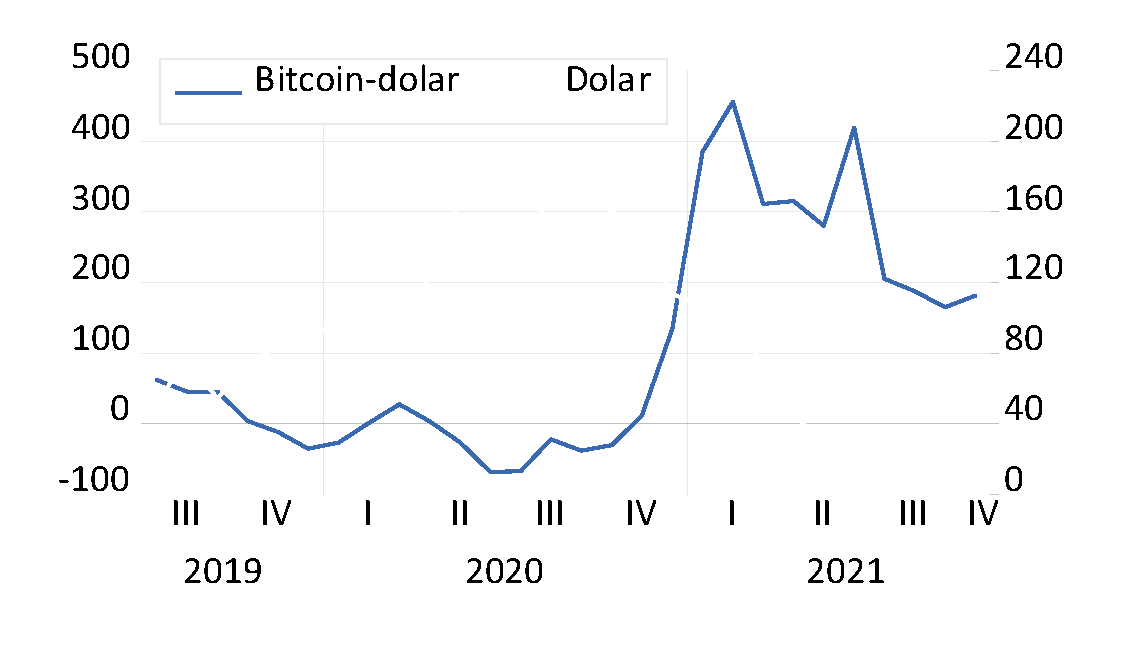
\includegraphics[width=1\textwidth]{images/C4/graph analysis/graph02_colores_03.pdf}
     \end{center}
\end{figure}

\note{
\begin{itemize}
    \item Con lo base de datos construida a partir de datos de google, se transforman las series de datos para obtener las variaciones anuales. \end{itemize}
}

\end{frame}
%----------

\begin{frame}
\frametitle{...respecto a la variación del \textcolor{orange}{tipo de cambio}.}

\begin{figure}[H]
    \begin{center}
     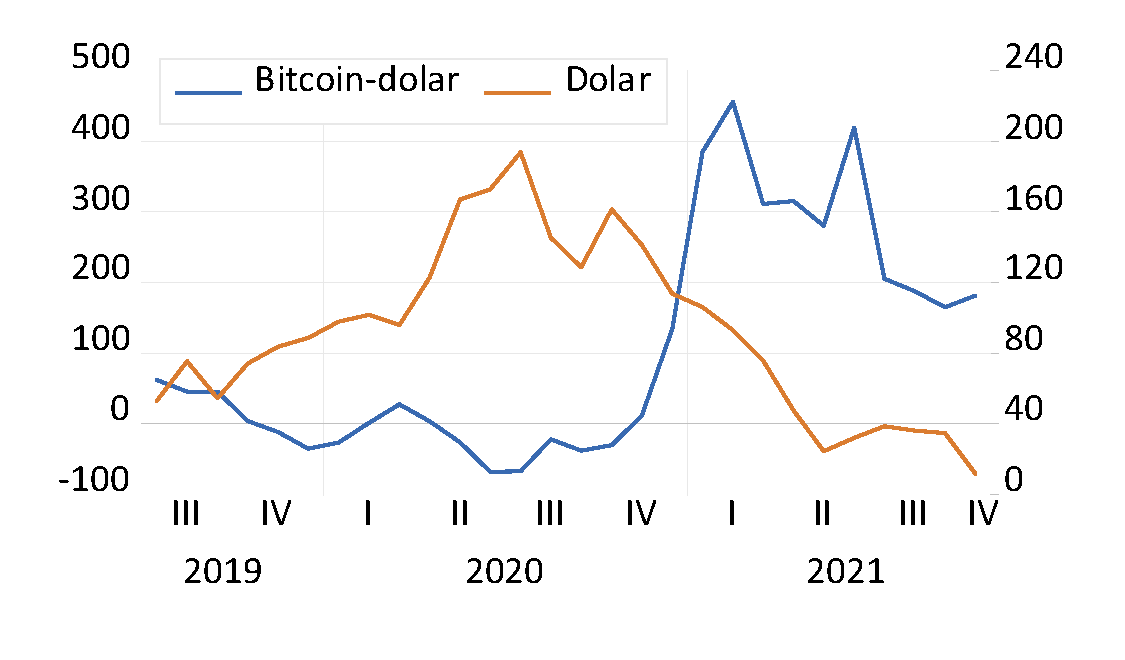
\includegraphics[width=1\textwidth]{images/C4/graph analysis/graph02_colores_04.pdf}
     \end{center}
\end{figure}

\note{
\begin{itemize}
    \item \item Se encuentra una asociación entre la variación en las búsquedas de google-bitcoin y el tipo de cambio. 
    \item Sin embargo, es necesario considerar, nuevamente, que las bases son de carácter prelimianar dado que no son fuentes oficiales provistas por proveedores locales, con lo cual los resultados dependen de la representatividad de las búsquedas en google. 
\end{itemize}
}

\end{frame}
%----------

\subsection{Resultados}
%---------------------

\begin{frame}{}

    \vspace{5mm}
    \begin{itemize}
        \setlength\itemsep{1em}
        \item[] La \textcolor{blue}{\textbf{conclusión principal}} a partir de la evaluación conceptual es que incrementos en la \textcolor{blue}{volatilidad de la demanda de bitcoin} pueden generar incrementos en la \textcolor{blue}{volatilidad en el tipo de cambio} ARS/USD. 
        \item[] De manera complementaria, la \textcolor{dgreen}{\textbf{evaluación conceptual}} indica que un incremento de la demanda de ciudadanos que \textcolor{dgreen}{demandaban dólares (pesos)} generará una \textcolor{dgreen}{apreciación (depreciación)} del tipo de cambio.

    \end{itemize}

\note{
\begin{itemize}
    \item Luego de realizar la evaluación conceptual y empírica en esta tercera parte de la investigación, se  llega a las siguientes conclusiones: (leer filmina)
    \item La conclusión general. Este resultado tiene como condición necesaria un incremento en el nivel de adopción generalizado de bitcoin en Argentina. 
    \item Evaluación empírica: hay que mejorar los datos
    \item No se observa volatilidad en la demanda a partir de google trends
    \item Se enceuntra asociación entre incrementos en las búsquedas de google bitocin y apreciación en el tipo de cambio (muy inicial). 
\end{itemize}
}
    
\end{frame}
%----------
